\section{Experiments and results}
\label{sec:experiments}

The programme has six experiments. E0 tests the pipeline; E1 and E2 address RQ1 and RQ2; E5
validates the LLM judges that label the trajectories. E3 addresses RQ3 with an observational
analysis and a forced-compaction pilot, and E4 addresses RQ4 offline, on the E1 and E2 trajectories.
The test of inherited drift planned for E3 and the monitor-degradation part of E4 were not run.

\subsection{E0: pilot}
\label{sec:e0}

The pilot ran the first two tasks with three candidate agent models, with no injection
(\textsf{none}, $k=0$) and with one sub-task of each source (\textsf{mix}). Its purpose was to check
that Claude Code could drive local models end to end and to measure the cost of an episode. It led to
four changes that are now part of the method:
\begin{itemize}
  \item \texttt{devstral} was dropped (tool calls emitted as text);
  \item the attribution header was disabled and the Ollama version pinned, which cut the latency of a
        turn from about 50\,s to typically a few seconds;
  \item the evaluator was isolated from the repository's pytest configuration;
  \item build artefacts were excluded from the diff. A single \texttt{pytestdebug.log} had
        inflated one pilot episode's out-of-scope ratio from 16\% to 89\%.
\end{itemize}

\subsection{E1: dose and source (RQ1, H1, H2)}
\label{sec:e1}

\paragraph{Design.} For each model, task and repetition we ran the $k=0$ baseline and every
combination of source $\in\{\textsf{user},\textsf{env},\textsf{text},\textsf{cascade},
\textsf{filler}\}$ and $k\in\{1,2,4\}$. That gives 16 cells $\times$ 12 tasks $\times$ 3 repetitions
$\times$ 2 models $=1{,}152$ episodes, all of which completed. An episode lasted a median of 14 minutes
for \texttt{qwen3-coder} and 26 for \texttt{gpt-oss}, with 43--48 tool calls on average.

\paragraph{Baseline.} Without sub-tasks the two models differ widely in competence, which is why
effects are reported as differences from each model's own baseline. \texttt{qwen3-coder} passes
77\% of the hidden requirements and fully meets the goal in 44\% of episodes; \texttt{gpt-oss}
passes 48\% and fully meets it in 31\%.

\begin{table}[t]
  \centering
  \caption{E1: hidden-test pass rate by model, source and number of injected sub-tasks $k$ (36
  episodes per cell; the $k=0$ column is the shared baseline). \emph{Slope}: change in pass rate per
  additional sub-task. \emph{vs.\ filler}: excess slope over the filler control. Holm-corrected:
  * $p<.05$, ** $p<.01$, *** $p<.001$.}
  \label{tab:e1}
  \small
  \fittable{\begin{tabular}{llcccccc}
\toprule
Model & Source & $k{=}0$ & $k{=}1$ & $k{=}2$ & $k{=}4$ & Slope per sub-task & vs.\ filler \\
\midrule
qwen3-coder 30B & User side-request & 0.77 & 0.79 & 0.73 & 0.78 & +0.001 & $-$0.003 \\
 & Environment (failing test) & 0.77 & 0.78 & 0.80 & 0.73 & $-$0.010 & $-$0.007 \\
 & Text (TODO/README) & 0.77 & 0.77 & 0.75 & 0.79 & +0.004 & $-$0.001 \\
 & Cascade (broken dependency) & 0.77 & 0.64 & 0.53 & 0.50 & $-$0.065** & $-$0.083*** \\
 & Filler (neutral control) & 0.77 & 0.76 & 0.78 & 0.78 & +0.005 & -- \\
\midrule
gpt-oss 20B & User side-request & 0.48 & 0.46 & 0.54 & 0.23 & $-$0.062 & $-$0.032 \\
 & Environment (failing test) & 0.48 & 0.53 & 0.57 & 0.50 & +0.003 & +0.026 \\
 & Text (TODO/README) & 0.48 & 0.50 & 0.62 & 0.51 & +0.009 & +0.031 \\
 & Cascade (broken dependency) & 0.48 & 0.47 & 0.41 & 0.24 & $-$0.062** & $-$0.041 \\
 & Filler (neutral control) & 0.48 & 0.49 & 0.40 & 0.46 & $-$0.008 & -- \\
\bottomrule
\end{tabular}
}
\end{table}

\begin{figure}[t]
  \centering
  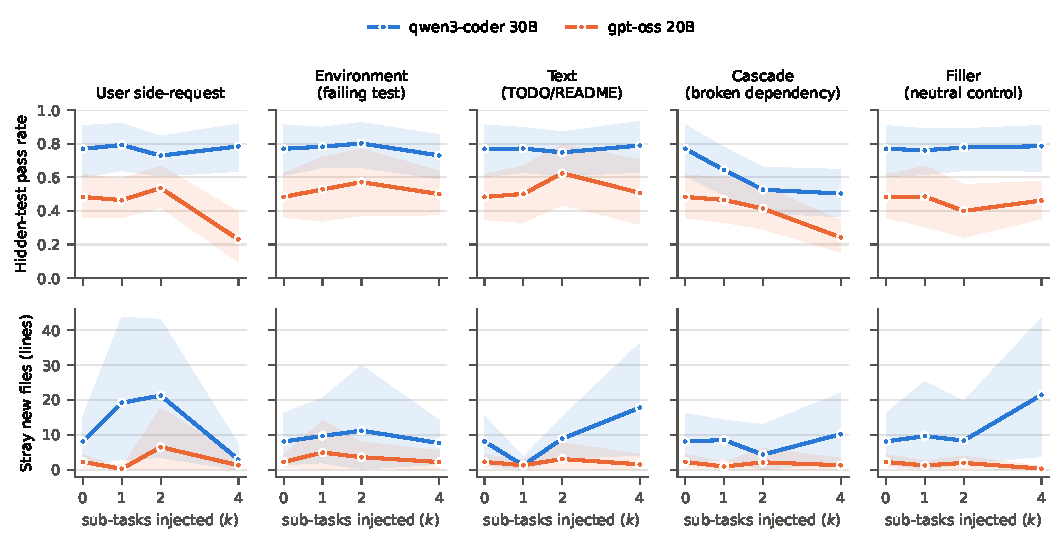
\includegraphics[width=\textwidth]{figures/e1_dose_response.pdf}
  \caption{E1 dose--response. Top: hidden-test pass rate; bottom: lines in stray new files left in
  the repository. Bands are 95\% task-cluster bootstrap intervals.}
  \label{fig:e1}
\end{figure}

\paragraph{Results.} Table~\ref{tab:e1} and Figure~\ref{fig:e1} summarise the outcome.
\begin{itemize}
  \item \textbf{Cascades are the only source that degrades the goal in both models.} With four
        broken dependencies, \texttt{qwen3-coder} falls from 0.77 to 0.50 (slope $-0.065$ per
        sub-task, Holm $p=.005$) and \texttt{gpt-oss} from 0.48 to 0.24 (slope $-0.062$, Holm
        $p=.005$). The share of episodes that fully meet the goal falls from 44\% to 8\% and from 31\%
        to 3\%. For \texttt{qwen3-coder} the loss is significantly larger than with the filler
        control (excess slope $-0.083$, Holm $p<.001$). For \texttt{gpt-oss} the difference points
        the same way ($-0.041$, uncorrected $p=.010$, Holm $p=.07$).
  \item \textbf{User side requests overload the weaker model.} \texttt{qwen3-coder} absorbs up to
        four requests without loss on the goal (0.73--0.79) and fulfils about 90\% of them.
        \texttt{gpt-oss} is unaffected up to $k=2$. At $k=4$ it loses on both fronts: the pass rate
        drops to 0.23 ($D_4=-0.25$, 95\% CI $[-0.46,-0.04]$) and only 40\% of the side requests are
        met. The linear trend is not significant after correction (uncorrected $p=.03$, Holm $p=.27$).
        The pattern is a threshold rather than a linear dose.
  \item \textbf{Distractors are largely ignored.} Failing unrelated tests (\textsf{env}) and
        instruction-like text (\textsf{text}) leave the pass rate within a few points of the
        baseline for both models. The one exception, a non-significant \emph{rise} for
        \texttt{gpt-oss} at $k=2$, is within the noise of the cell. Edits to existing out-of-scope
        files stay below 3.5\% of changed lines in every cell, so neither model acted on planted
        instructions that pointed outside the scope. Inside the scope the judge panel of E5 finds
        the same: at most 6.4\% of segments in any cell are labelled as work on a distractor
        (Section~\ref{sec:judge-results}).
  \item \textbf{Longer context alone does not hurt.} The filler control is flat for both models,
        so the losses above cannot be attributed to the added length of the pauses.
  \item \textbf{Stray files vary but show no trend.} \texttt{qwen3-coder} leaves 1--21 lines of
        debugging scripts per episode on average and \texttt{gpt-oss} 0--6. No slope is significant.
\end{itemize}
Two process observations matter for E3 and E4. \texttt{qwen3-coder} triggers Claude Code's automatic
compaction in 19\% of episodes and \texttt{gpt-oss} in only 1\%, with no difference across sources.
\texttt{gpt-oss} modifies a protected file in 13\% of episodes, including 19\% of baseline
episodes, against 0.5\% for \texttt{qwen3-coder}. These modifications are not driven by the
failing tests of the \textsf{env} source (11\%).

\paragraph{Against the hypotheses.} H1 holds only for cascades, and for user requests in the
weaker model at the highest dose. It does not hold for distractors: in this setting the number of
sub-tasks matters much less than their kind. H2 is partly supported:
\begin{itemize}
  \item As predicted, sanctioned user requests produce \emph{incompletion} rather than scope
        violation, but only for \texttt{gpt-oss} and only at $k=4$.
  \item Contrary to H2, \textsf{text} distractors do not produce scope violations, and \textsf{env}
        obstacles do not produce effort displacement onto protected tests.
  \item Also contrary to H2, \textsf{cascade} sub-tasks are the \emph{most} damaging, not the least.
\end{itemize}
The cascade result needs care. By construction a cascade that the agent fails to repair lowers the
score even if the agent never stops pursuing $\Gz$, so part of this loss is unresolved necessary
work rather than drift away from the goal. The judge-based measures of
Section~\ref{sec:judge-results} give a partial answer: for \texttt{qwen3-coder} up to 18\% of
segments go to work off the goal under cascades, none of it labelled as distracting work, and for
\texttt{gpt-oss} the share does not rise at all. Whether each broken dependency was
eventually fixed is not among the judged fields and remains open.

\subsection{E2: harness mitigations (RQ2, H3)}
\label{sec:e2}

\paragraph{Design.} E2 fixes the load at one sub-task of each source (\textsf{mix}: one user
request at the first pause, one \textsf{env}, one \textsf{text} and one \textsf{cascade} injection
in the repository) and varies the harness. It compares five conditions on \texttt{qwen3-coder}
(12 tasks $\times$ 3 repetitions each, 180 episodes):
\begin{itemize}
  \item \emph{no mitigation};
  \item a \emph{goal re-anchoring hook}: a \texttt{UserPromptSubmit} hook that appends the original
        goal, verbatim, to every new message;
  \item a \emph{stop-hook checklist}: a \texttt{Stop} hook that blocks the first attempt to stop in
        each turn and asks the agent to check each numbered requirement of the original goal;
  \item \emph{sub-agent delegation}: an appended system instruction to hand any sub-task outside the
        original goal to a sub-agent through the \texttt{Task} tool;
  \item a \emph{task list}: Claude Code's task-list tools enabled, plus an instruction to record each
        requirement and each new sub-task and to check the list before finishing.
\end{itemize}
The two hook conditions act outside the model and are deterministic. The last two depend on the
model following an instruction. Hooks are disabled during the probe, so that goal recall is never
answered with the hook's help.

\begin{table}[t]
  \centering
  \caption{E2: mitigations under a fixed load of four sub-tasks (\textsf{mix}),
  \texttt{qwen3-coder}, 36 episodes per condition. $\Delta$: difference in hidden pass rate from no
  mitigation, with 95\% task-cluster bootstrap interval. No difference is significant after Holm
  correction.}
  \label{tab:e2}
  \small
  \fittable{\begin{tabular}{lcccccc}
\toprule
Condition & \makecell{Hidden\\pass} & \makecell{$\Delta$ vs.\ none\\{}[95\% CI]} & \makecell{Goal\\fully met} & \makecell{Side request\\met} & \makecell{Stray\\lines} & \makecell{Tool\\calls} \\
\midrule
No mitigation & 0.630 & -- & 0.14 & 0.81 & 8.2 & 48.2 \\
Goal re-anchoring hook & 0.647 & +0.018 [$-$0.03, +0.08] & 0.11 & 0.89 & 6.6 & 47.8 \\
Stop-hook checklist & 0.620 & $-$0.010 [$-$0.08, +0.06] & 0.17 & 0.86 & 11.4 & 53.2 \\
Sub-agent delegation & 0.682 & +0.052 [$-$0.01, +0.12] & 0.14 & 0.83 & 9.4 & 51.0 \\
Task list & 0.685 & +0.055 [+0.00, +0.11] & 0.14 & 0.81 & 19.7 & 56.4 \\
\bottomrule
\end{tabular}
}
\end{table}

\begin{figure}[t]
  \centering
  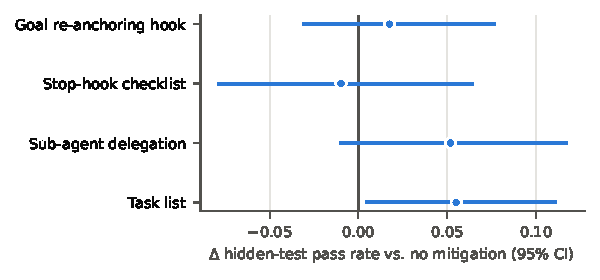
\includegraphics[width=0.62\textwidth]{figures/e2_mitigations.pdf}
  \caption{E2: effect of each mitigation on the hidden pass rate (95\% task-cluster bootstrap
  intervals).}
  \label{fig:e2}
\end{figure}

\paragraph{Results.} Under the mixed load \texttt{qwen3-coder} passes 63\% of the hidden requirements
without mitigation, against 77\% with no sub-tasks in E1. No mitigation changes this significantly
(Table~\ref{tab:e2}, Figure~\ref{fig:e2}):
\begin{itemize}
  \item The task list and sub-agent delegation show the largest point estimates: $+0.055$
        (95\% CI $[+0.004, +0.112]$) and $+0.052$ ($[-0.010, +0.118]$). Neither survives correction
        (Holm $p=.28$ and $p=.45$).
  \item The re-anchoring hook fired on every message, six times per episode, yet changed the goal
        pass rate by only $+0.018$. It raised the completion of the user's side request from 81\% to
        89\%.
  \item The stop-hook checklist had no effect ($-0.010$) and fired only 1.4 times per episode,
        because most segments end at the turn limit rather than by the agent deciding to stop.
\end{itemize}
How far each mitigation was taken up differs sharply:
\begin{itemize}
  \item Despite the instruction, \texttt{qwen3-coder} delegated to a sub-agent in only 2 of 36
        episodes.
  \item It used the task list in 24 of 36 episodes.
  \item The task list was also the most expensive condition: 56 tool calls against 48 without
        mitigation, and the most stray new lines (20 against 8).
\end{itemize}

\paragraph{Against the hypotheses.} H3 is not supported in its strong form. Deterministic hooks did
not outperform instruction-based mitigations; if anything the ordering is reversed. Their weakness
is not that the model ignored them, since the re-anchoring hook fired every time. They inject
information the model already has at moments that do not coincide with the loss. The
instruction-based conditions depend on compliance, which was low for delegation. Within this power
(36 episodes per condition, intervals of about $\pm 0.06$), no lightweight harness change removes
the loss caused by the mixed load.

\subsection{E5: judge validation}
\label{sec:e5}

The trajectory-level measures (effort share, goal recall, goal replacement, report fidelity) rely on
LLM judges. No human annotator was available, so E5 replaces human labels with a panel of three
judges from three model families, none of which is an agent under test: \texttt{gpt-oss:120b}
with medium reasoning effort, and \texttt{mistral-small3.2:24b} and \texttt{llama3.3:70b} without
reasoning.
\texttt{gpt-oss:120b} shares a family with the \texttt{gpt-oss:20b} agent, so every agreement figure
is also reported per agent model. Each judge labels every segment of every E1/E2 episode (7{,}991
segments) with one of five labels (\textsf{GOAL}, \textsf{SANCTIONED}, \textsf{NECESSARY},
\textsf{DISTRACTOR}, \textsf{NONE}) and every episode (1{,}332) on whether its final summary claims
completion and what it presents as the main accomplishment. Items are blinded to the agent model and
the outcome, but not to the condition: the task card shows the injected sub-tasks, which the judge
needs in order to tell sanctioned from distracting work. One stylistic difference cannot be hidden:
\texttt{qwen3-coder} runs pytest in verbose mode. The panel majority labels each item; items on
which all three judges disagree get no label and are excluded. The criterion is Fleiss'
$\kappa\ge 0.6$. A panel without human labels measures reliability, not validity: the labels show
that three independent models read the trajectories in the same way, not that they read them
correctly.

The first codebook passed on a pilot sample of 60 segments ($\kappa=0.71$) but not on the full set
($\kappa=0.44$, 95\% CI 0.42--0.45; \texttt{claims\_complete} $\kappa=0.65$). Reading the
disagreements showed two causes. First, the codebook had two pairs of rules that contradicted each
other, on wrap-up segments (re-running passing tests) and on read-only orientation. Second, one judge
labelled segments by the session context rather than by the actions in the segment. Codebook v2
states that the label follows the actions in the segment, sharpens \textsf{NONE} and adds three
worked examples. On a held-out stratified sample of 260 segments, v2 raised $\kappa$ from 0.44 to
0.57 for the five labels and from 0.53 to 0.67 for the distinction that defines drift: work leaving
the goal (\textsf{SANCTIONED}, \textsf{NECESSARY} or \textsf{DISTRACTOR}) versus the rest. We
therefore use this binary label as the primary segment measure and the five labels as a secondary
one. This choice was made after seeing the held-out agreement. In the held-out sample, reliability
is lower on \texttt{qwen3-coder} episodes ($\kappa=0.54$ for the binary label), where the residual disagreement
is between \textsf{GOAL} and \textsf{NONE}.

On the full set (7{,}990 segments with a complete panel), codebook v2 gives $\kappa=0.667$ (95\% CI
0.647--0.686, raw agreement 0.93) for the binary label, matching the held-out estimate: 0.723 on
\texttt{gpt-oss:20b} episodes and 0.615 on \texttt{qwen3-coder} episodes. The five labels reach
0.575 (0.559--0.591) and \texttt{claims\_complete} 0.658 (0.614--0.701). Recall ($\kappa=0.17$) and
the main accomplishment ($\kappa=0.45$) stay below the criterion: recall is not used, and goal
replacement is reported only as exploratory. The three judges disagree completely on 58 of 7{,}991
segments (0.7\%; 41 of 4{,}536 for \texttt{qwen3-coder} and 17 of 3{,}455 for \texttt{gpt-oss}) and
on 5 of 1{,}332 \texttt{claims\_complete} labels; these labels are excluded.

In 3 of the 1{,}332 episodes (0.2\%, all \texttt{gpt-oss:20b} on two tasks) the agent ran
\texttt{grep -R ..} from its working directory and so read the harness's own log files. None of
them read the episode specification that names the condition. Agent model names that reached two
judge items this way were replaced by a placeholder before judging.

\subsection{Judge-based measures in E1 and E2}
\label{sec:judge-results}

Each episode yields four judge-based measures:
\begin{itemize}
  \item the \emph{off-goal share}, the fraction of its labelled segments marked \textsf{SANCTIONED},
        \textsf{NECESSARY} or \textsf{DISTRACTOR} (primary);
  \item the \emph{distractor share}, the fraction marked \textsf{DISTRACTOR}, which is the
        illegitimate part of the off-goal work;
  \item \emph{over-claiming}: the final summary claims completion while at least one hidden test
        fails;
  \item \emph{goal replacement}: the main accomplishment named in the summary is not the goal
        (exploratory).
\end{itemize}
Table~\ref{tab:e5e1} and Figure~\ref{fig:e5} report E1, Table~\ref{tab:e5e2} reports E2. Intervals
are 95\% task-cluster bootstrap intervals with 36 episodes per cell, as in
Section~\ref{sec:analysis}, but they are \emph{not} corrected for multiplicity: these measures
were added after the outcome analysis and span 40 E1 cells and 4 E2 contrasts, so an isolated
interval that just excludes zero should be read with caution.

\begin{table}[t]
  \centering
  \caption{E1, judge-based measures by model, source and $k$ (36 episodes per cell; $k=0$ is the
  shared baseline). Off-goal share: mean fraction of an episode's segments that the judge panel
  labels \textsf{SANCTIONED}, \textsf{NECESSARY} or \textsf{DISTRACTOR}. Over-claim rate: fraction
  of episodes whose final summary claims completion while a hidden test fails.}
  \label{tab:e5e1}
  \small
  \fittable{\begin{tabular}{llcccccccc}
\toprule
 & & \multicolumn{4}{c}{Off-goal share (incl.\ sanctioned/necessary)} & \multicolumn{4}{c}{Over-claim rate} \\
Model & Source & $k{=}0$ & $k{=}1$ & $k{=}2$ & $k{=}4$ & $k{=}0$ & $k{=}1$ & $k{=}2$ & $k{=}4$ \\
\midrule
qwen3-coder 30B & User side-request & 0.00 & 0.16 & 0.27 & 0.53 & 0.42 & 0.47 & 0.56 & 0.44 \\
 & Environment (failing test) & 0.00 & 0.00 & 0.00 & 0.01 & 0.42 & 0.53 & 0.33 & 0.54 \\
 & Text (TODO/README) & 0.00 & 0.00 & 0.01 & 0.00 & 0.42 & 0.50 & 0.50 & 0.34 \\
 & Cascade (broken dependency) & 0.00 & 0.05 & 0.10 & 0.18 & 0.42 & 0.75 & 0.81 & 0.78 \\
 & Filler (neutral control) & 0.00 & 0.01 & 0.00 & 0.01 & 0.42 & 0.56 & 0.56 & 0.44 \\
\midrule
gpt-oss 20B & User side-request & 0.08 & 0.29 & 0.38 & 0.62 & 0.50 & 0.61 & 0.58 & 0.76 \\
 & Environment (failing test) & 0.08 & 0.07 & 0.09 & 0.10 & 0.50 & 0.56 & 0.50 & 0.56 \\
 & Text (TODO/README) & 0.08 & 0.06 & 0.08 & 0.03 & 0.50 & 0.56 & 0.53 & 0.61 \\
 & Cascade (broken dependency) & 0.08 & 0.09 & 0.07 & 0.06 & 0.50 & 0.78 & 0.81 & 0.81 \\
 & Filler (neutral control) & 0.08 & 0.05 & 0.05 & 0.03 & 0.50 & 0.53 & 0.67 & 0.69 \\
\bottomrule
\end{tabular}
}
\end{table}

\begin{figure}[t]
  \centering
  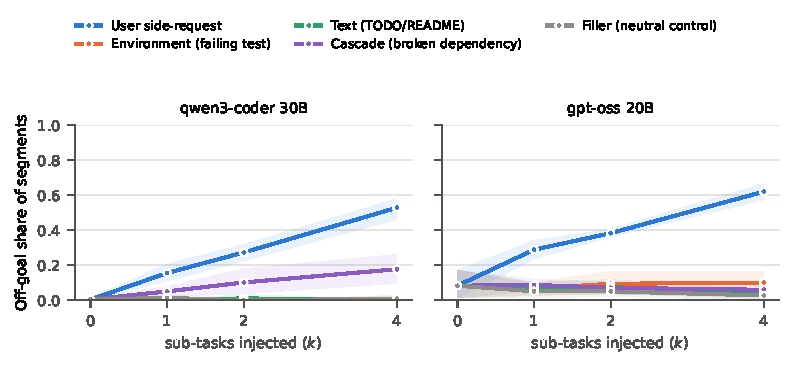
\includegraphics[width=0.85\textwidth]{figures/e5_off_share.pdf}
  \caption{E1: off-goal share of segments by source and number of injected sub-tasks. Bands are
  95\% task-cluster bootstrap intervals.}
  \label{fig:e5}
\end{figure}

\begin{table}[t]
  \centering
  \caption{E2, judge-based measures under the \textsf{mix} load, \texttt{qwen3-coder}, 36 episodes
  per condition. $\Delta$: difference from no mitigation, with 95\% task-cluster bootstrap interval
  (not corrected for multiplicity).}
  \label{tab:e5e2}
  \small
  \fittable{\begin{tabular}{llcccc}
\toprule
Model & Condition & \makecell{Off-goal share\\(incl.\ sanctioned)} & \makecell{$\Delta$ vs.\ none\\{}[95\% CI]} & \makecell{Over-claim\\rate} & \makecell{$\Delta$ vs.\ none\\{}[95\% CI]} \\
\midrule
qwen3-coder 30B & No mitigation & 0.19 & -- & 0.69 & -- \\
 & Goal re-anchoring hook & 0.21 & +0.02 [$-$0.03, +0.06] & 0.89 & +0.20 [+0.08, +0.36] \\
 & Stop-hook checklist & 0.20 & +0.01 [$-$0.03, +0.06] & 0.69 & +0.01 [$-$0.13, +0.14] \\
 & Sub-agent delegation & 0.19 & $-$0.00 [$-$0.05, +0.04] & 0.69 & +0.01 [$-$0.19, +0.21] \\
 & Task list & 0.14 & $-$0.05 [$-$0.11, +0.00] & 0.75 & +0.06 [$-$0.08, +0.21] \\
\bottomrule
\end{tabular}
}
\end{table}

\paragraph{Off-goal work follows the user's requests.} The off-goal share rises with $k$ only for
user side requests. For \texttt{qwen3-coder} it goes from 0.005 at baseline to 0.16, 0.27 and 0.53
at $k=1,2,4$; for \texttt{gpt-oss} from 0.08 to 0.29, 0.38 and 0.62. At $k=4$ the difference from
baseline is $D_4=+0.52$ $[0.45, 0.58]$ and $+0.54$ $[0.46, 0.62]$, and the difference from the filler
control at the same $k$ is of the same size ($+0.52$ $[0.45, 0.57]$ and $+0.59$ $[0.53, 0.65]$).
Cascades raise the share for \texttt{qwen3-coder} only: 0.18 at $k=4$, $D_4=+0.17$ $[0.09, 0.26]$.
For \texttt{gpt-oss} cascades stay at baseline. The \textsf{env}, \textsf{text} and \textsf{filler}
conditions stay within $\pm0.06$ of baseline in both models, with intervals that include zero. A few
\texttt{qwen3-coder} intervals only touch zero at one end, such as $+0.005$ $[0, 0.014]$ with four
\textsf{env} injections, and the amounts are negligible.

\paragraph{Almost none of it is distraction.} The distractor share is close to zero everywhere. Its
largest value is 0.064, for \texttt{gpt-oss} with four \textsf{env} injections, and for
\texttt{qwen3-coder} it is zero in all but two cells. The agents rarely acted on planted
\texttt{TODO}/README text or on unrelated failing tests in a way the judges label as distracting
work. The off-goal work they did is almost entirely the work the user asked for or the repairs the
goal needed.

\paragraph{Over-claiming is common and rises with cascades.} At baseline the final summary claims
completion while a hidden test fails in 42\% of \texttt{qwen3-coder} episodes and 50\% of
\texttt{gpt-oss} episodes. Cascades raise this in both models at every dose. For
\texttt{qwen3-coder} the rate is 0.75, 0.81 and 0.78 at $k=1,2,4$ ($D_k=+0.33$ $[0.11, 0.58]$,
$+0.39$ $[0.17, 0.61]$, $+0.36$ $[0.11, 0.64]$). For \texttt{gpt-oss} it is 0.78, 0.81 and 0.81
($+0.28$ $[0.17, 0.39]$, $+0.31$ $[0.11, 0.50]$, $+0.31$ $[0.08, 0.50]$). Against the filler control
the excess is clear only for \texttt{qwen3-coder} at $k=2$ and $k=4$ ($+0.25$ $[0.03, 0.50]$ and
$+0.33$ $[0.08, 0.58]$), because the filler itself raises over-claiming in some cells
(\texttt{qwen3-coder} $k=1$: $+0.14$ $[0.03, 0.25]$; \texttt{gpt-oss} $k=4$: $+0.19$
$[0.03, 0.33]$). Part of the cascade effect is mechanical: cascades lower the pass rate, so more
episodes have a failing test that a claim of completion can contradict. With four side requests
\texttt{gpt-oss} over-claims in 0.76 of episodes, but the interval of the difference includes zero
($+0.26$ $[-0.01, 0.55]$). The only other interval that excludes zero is a \emph{lower} rate for
\texttt{qwen3-coder} with two \textsf{env} injections than with filler ($-0.22$ $[-0.39, -0.06]$).

\paragraph{Goal replacement (exploratory).} With the caveat of its low reliability ($\kappa=0.45$),
the summary names something other than the goal as the main accomplishment in 8\% of baseline
\texttt{qwen3-coder} episodes and 19\% of \texttt{gpt-oss} episodes, and no E1 cell differs from
baseline with an interval that excludes zero.

\paragraph{E2.} No mitigation changes the off-goal share under the mixed load (0.19 without
mitigation). The task list has the largest point estimate, $-0.05$ $[-0.11, 0.00]$. The re-anchoring
hook increases over-claiming: 0.89 of its episodes claim completion with a hidden test failing,
against 0.69 without mitigation ($+0.20$ $[0.08, 0.36]$). The other mitigations leave over-claiming
unchanged. We have not examined why the hook has this effect.

\subsection{E3: compaction (RQ3, H4)}
\label{sec:e3}

When the context approaches its limit, Claude Code replaces the conversation with a summary written
by the model, and whatever the summary leaves out is lost for the rest of the session. E3 asks
whether this step changes how the agent divides its effort between the goal and the sub-tasks. It
has two parts: an observational comparison of the E1 and E2 episodes in which compaction happened
on its own, and a small pilot in which compaction is forced. The planned test of inherited drift was
not run, for the reason given at the end of this section.

\begin{table}[t]
  \centering
  \caption{E3, observational: \texttt{qwen3-coder} episodes of E1 and E2 with automatic compaction
  against episodes without it. Control episodes are re-weighted to the compacted episodes' mix of
  experiment, source, $k$ and condition. The last row compares segments after and before the first
  compaction within the same episodes, excluding the segment in which it occurred. Intervals are
  95\% task-cluster bootstrap intervals. The comparison is correlational.}
  \label{tab:e3obs}
  \small
  \fittable{\begin{tabular}{llcccc}
\toprule
Contrast & Measure & $n$ & \makecell{Compacted\\/ after} & \makecell{Matched none\\/ before} & \makecell{Difference\\{}[95\% CI]} \\
\midrule
compacted vs matched none & hidden pass & 135 & 0.46 & 0.77 & $-$0.31 [$-$0.43, $-$0.02] \\
compacted vs matched none & over claim & 135 & 0.36 & 0.63 & $-$0.26 [$-$0.42, $-$0.08] \\
compacted vs matched none & off share & 135 & 0.08 & 0.11 & $-$0.03 [$-$0.05, $-$0.00] \\
after vs before first compaction & off share & 18 & 0.06 & 0.10 & $-$0.04 [$-$0.25, +0.01] \\
\bottomrule
\end{tabular}
}
\end{table}

\paragraph{Spontaneous compaction.} In E1 and E2, 135 \texttt{qwen3-coder} episodes triggered
automatic compaction. Against non-compacted episodes from the same experiment, source, $k$ and
condition (Table~\ref{tab:e3obs}), they pass fewer hidden tests, 0.46 against 0.77 (difference
$-0.31$, 95\% CI $[-0.43, -0.02]$), and they over-claim less often, 0.36 against 0.63 ($-0.26$
$[-0.42, -0.08]$): their final summaries more often admit that the work is unfinished. Their
off-goal share is slightly lower (0.08 against 0.11). In the 18 episodes where segments on both
sides of the first compaction could be compared, the off-goal share is 0.06 after it and 0.10
before, with an interval from $-0.25$ to $+0.01$. These differences cannot be read causally.
Compaction happens when the context fills up, that is in long episodes in which the agent is
struggling, and such episodes would fail more often with or without it.

\paragraph{Forced compaction: design.} The pilot uses \texttt{qwen3-coder} with four user side
requests ($k=4$), the condition in which the off-goal share is highest and the goal still mostly
met. It compares two arms of 12 tasks $\times$ 3 repetitions (36 episodes each): in one the harness
sends Claude Code's \texttt{/compact} command right after the segment of the second pause, before
the third side request; in the other it does not. The command works in headless mode. Up to that point the two
arms are identical, so the off-goal share of the pre-compaction segments (initial segment and first
two pauses) is a placebo that should show no difference; the post-compaction segments are the third
and fourth pauses and the final segment. The judge panel labelled the pilot's 432 segments and 72
episodes with codebook v2. Agreement on the binary off-goal label is $\kappa=0.632$ (95\% CI
0.575--0.688), above the criterion, and 0.588 for the five labels. \texttt{claims\_complete} reaches
only 0.562 (0.37--0.73), below the criterion, so over-claiming in E3 carries that caveat. Recall
(0.26) is not used, and the main accomplishment (0.31) makes goal replacement exploratory only.

\begin{table}[t]
  \centering
  \caption{E3, forced-compaction pilot: \texttt{qwen3-coder}, four user side requests, 12 tasks
  $\times$ 3 repetitions per arm, \texttt{/compact} sent after the second pause. Difference:
  compaction minus no compaction, with 95\% task-cluster bootstrap interval. Off-goal share:
  segments labelled \textsf{SANCTIONED}, \textsf{NECESSARY} or \textsf{DISTRACTOR}; with this source
  it consists mostly of work on the user's own requests. Pre-compaction segments are a placebo.
  Over-claim rests on \texttt{claims\_complete}, whose agreement on E3 is below the criterion
  ($\kappa=0.56$); goal replacement is exploratory ($\kappa=0.31$). The pilot is exploratory.}
  \label{tab:e3pilot}
  \small
  \fittable{\begin{tabular}{lccc}
\toprule
Measure & Compaction ($n$) & No compaction ($n$) & Difference [95\% CI] \\
\midrule
Hidden-test pass & 0.72 (36) & 0.77 (36) & $-$0.05 [$-$0.11, +0.00] \\
Side-request pass & 0.90 (36) & 0.84 (36) & +0.06 [$-$0.01, +0.15] \\
Out-of-scope edits (existing files) & 0.00 (36) & 0.00 (36) & $-$0.00 [$-$0.01, +0.00] \\
Protected file modified (share) & 0.03 (36) & 0.00 (36) & +0.03 [+0.00, +0.08] \\
Automatic compactions (beyond the forced one) & 0.08 (36) & 0.17 (36) & $-$0.08 [$-$0.28, +0.08] \\
Over-claim & 0.43 (35) & 0.42 (36) & +0.01 [$-$0.14, +0.17] \\
Off-goal share, all segments & 0.59 (36) & 0.50 (36) & +0.09 [+0.06, +0.12] \\
Off-goal share, pre-compaction segments (placebo) & 0.54 (36) & 0.49 (36) & +0.05 [$-$0.01, +0.10] \\
Off-goal share, post-compaction segments & 0.63 (36) & 0.50 (36) & +0.13 [+0.06, +0.20] \\
Goal replaced (exploratory) & 0.47 (36) & 0.17 (36) & +0.31 [+0.11, +0.53] \\
\bottomrule
\end{tabular}
}
\end{table}

\paragraph{Forced compaction: results.} Table~\ref{tab:e3pilot} gives the outcome. After the
compaction the agent spent more of its segments off the goal: 0.63 against 0.50 in the
post-compaction segments ($+0.13$ $[+0.06, +0.20]$). Under this source off-goal work is almost all
\textsf{SANCTIONED}, the user's own side requests, so the increase means that after compaction the
agent gave more of its effort to the third and fourth requests relative to the goal. It does not
mean that it turned to distractors. The outcomes point the same way, with intervals that touch
zero: the hidden pass rate fell from 0.77 to 0.72 ($-0.05$ $[-0.11, +0.00]$) and the side-request
pass rate rose from 0.84 to 0.90 ($+0.06$ $[-0.01, +0.15]$). Over-claiming did not change (0.43
against 0.42). Edits to existing out-of-scope files were negligible in both arms (below 0.3\% of changed
lines), and one compacted episode modified a protected file. The placebo is not clean: the pre-compaction segments, identical by design, differ
by $+0.05$ $[-0.01, +0.10]$, so part of the post-compaction difference may be an imbalance between
the arms that was there before the compaction. The post-compaction difference is larger than the
placebo, but by less than the width of either interval. As an exploratory signal, the judges more
often read the final summary of a compacted episode as presenting a side request as the main
accomplishment (0.47 against 0.17), but their agreement on that field is too low to build on.

\paragraph{Inherited drift was not run.} The second part of E3 was to resume \texttt{qwen3-coder}
from trajectory prefixes produced by a weaker model under heavy load, in the spirit of
\citet{menon2026inherited}. Smoke tests with \texttt{qwen2.5:7b}, the planned weak model, showed
that it writes some tool calls as plain text, which Claude Code does not execute, and that it
claims completion falsely. Its prefixes would therefore be broken trajectories rather than drifted
ones, and a stronger model resuming them would inherit failed actions, not a displaced goal. The
lesson for the design is that the weak model must use the harness competently, so that its prefixes
differ from a strong model's in where they go rather than in whether they work. This test is left to
future work.

\paragraph{Against the hypotheses.} H4 is partly supported, on pilot evidence. Forced compaction
moved effort in the remaining segments away from the goal and towards the side requests, with a
small and uncertain cost to goal completion. It did not produce the constraint violations H4
predicted, and goal recall could not be measured because the judges do not agree on it. Inheritance
was not tested. With one model, one source and twelve tasks, the result is a direction for a larger
experiment, not an estimate.

\subsection{E4: the supervisor's view (RQ4, H5)}
\label{sec:e4}

E4 asks what a human supervisor could learn from the E1 and E2 trajectories, and at what cost. It
needs no new runs: it uses the episodes, their diffs and test results, the final summaries and the
v2 panel labels. It has two parts, report fidelity and a simulated supervisor. The third planned
part, whether a drift monitor degrades on longer transcripts \citep{martin2026classifier}, is left
to future work.

\paragraph{Report fidelity.} Over-claiming, a summary that claims completion while a hidden test
fails, is reported in Section~\ref{sec:judge-results}: 42\% of \texttt{qwen3-coder} and 50\% of
\texttt{gpt-oss} baseline episodes, 75--81\% under cascades. The second measure is \emph{omitted
changes}: a pre-existing out-of-scope file, or a protected file, that the diff changes but whose path
or base name does not appear in the final summary. It is a deterministic string match with no judge.
The match is strict, so a summary that describes a change without naming the file counts as an
omission, and the rates are upper bounds. \texttt{qwen3-coder} seldom touches such files, and its
omission rates stay between 0 and 8\% in every E1 cell (11\% with sub-agent delegation in E2).
\texttt{gpt-oss} touches them more often: 14\% of its baseline episodes omit a changed out-of-scope
file and 11\% a changed protected file, rising to 28\% for out-of-scope files with four \textsf{env}
injections. When such a file was changed, the summary usually did not name it: in 14 of the 16
\texttt{gpt-oss} cells it was omitted in at least half of those episodes, and in the two
\texttt{qwen3-coder} user-request cells where such changes occurred in 50\% and 75\%. These conditional rates rest on few
episodes and have wide intervals.

\paragraph{Supervisor simulation: design.} Each episode is replayed segment by segment, and a
simulated supervisor sees the panel's majority label of every segment it reviews. Three policies are
compared:
\begin{itemize}
  \item \emph{P0}: the supervisor reads only the final summary (one review) and is alerted if it
        does not claim completion;
  \item \emph{P1}: the supervisor reviews after each of the six segments (six reviews), is alerted at
        the first segment not labelled \textsf{GOAL}, and also reads the summary;
  \item \emph{P2}: a monitor alerts on segments labelled \textsf{DISTRACTOR} or \textsf{NONE}, and
        the supervisor reviews only the alerts.
\end{itemize}
The target is a failing episode, one with a hidden pass rate below 1: 525 of the 756
\texttt{qwen3-coder} episodes and 444 of the 576 \texttt{gpt-oss} episodes. The benefit of a policy
is the share of failing episodes it flags before the final segment, when the supervisor could still
redirect the agent; its cost is the number of reviews per episode; a false alarm is an alert in a
passing episode. The simulated supervisor applies the panel labels without error, so the results
are upper bounds for this information, not a user study. P1's alerts include legitimate detours,
sanctioned or necessary, which is why it raises false alarms in passing episodes.

\begin{table}[t]
  \centering
  \caption{E4, simulated supervisor on E1 and E2, all episodes per model (by group in Appendix~\ref{app:e4}, Table~\ref{tab:e4full}). Failing: hidden pass rate below 1. P0 reads only
  the final summary and is alerted if it does not claim completion; P1 reviews after all six
  segments and is alerted at the first segment not labelled \textsf{GOAL}; P2 is a monitor that
  alerts on \textsf{DISTRACTOR} or \textsf{NONE} segments (reviews = alerts). Early: flagged before
  the final segment. False alarm: an alert in a passing episode. The supervisor is assumed to apply
  the panel labels exactly, so the figures are upper bounds.}
  \label{tab:e4}
  \small
  \fittable{% "All episodes" rows of results/analysis/tables/e4_supervisor.tex (full table in the appendix).
\begin{tabular}{lcccccccccc}
\toprule
 & & & \multicolumn{3}{c}{Reviews / episode} & \multicolumn{3}{c}{Failing flagged early (\%)} & \multicolumn{2}{c}{False alarms (\%)} \\
Model & $n$ & fail & P0 & P1 & P2 & P0 & P1 & P2 & P1 & P2 \\
\midrule
qwen3-coder 30B & 756 & 525 & 1.0 & 6.0 & 0.7 & 0 & 56 & 19 & 77 & 62 \\
gpt-oss 20B & 576 & 444 & 1.0 & 6.0 & 0.3 & 0 & 44 & 18 & 55 & 28 \\
\bottomrule
\end{tabular}
}
\end{table}

\begin{figure}[t]
  \centering
  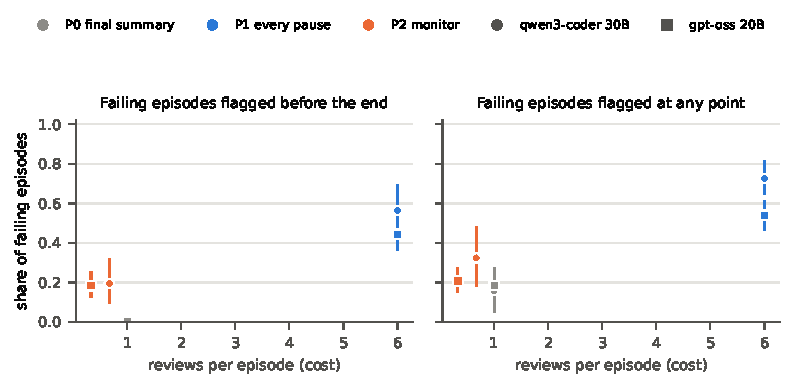
\includegraphics[width=\textwidth]{figures/e4_supervisor.pdf}
  \caption{E4: share of failing episodes flagged before the end (left) and at any point (right)
  against reviews per episode, for the three policies and both models. Bars are 95\% task-cluster
  bootstrap intervals.}
  \label{fig:e4}
\end{figure}

\paragraph{Supervisor simulation: results.} Table~\ref{tab:e4} and Figure~\ref{fig:e4} give the
results.
\begin{itemize}
  \item \emph{P0} cannot flag anything early by construction. At the end it flags 16\% of the
        failing \texttt{qwen3-coder} episodes and 18\% of the \texttt{gpt-oss} ones: in most of
        the rest the summary claims completion. False alarms are 5\% and 12\%.
  \item \emph{P1} flags 56\% (95\% CI 45--70\%) and 44\% (36--54\%) of failing episodes early, and
        73\% and 54\% at some point, at six reviews per episode. False alarms are 77\% and 55\%.
        Most of its alerts are detours the user asked for: with user side requests it flags
        94--96\% of failing episodes early, and also 98--100\% of the passing ones
        (Table~\ref{tab:e4full}).
  \item \emph{P2} costs 0.67 and 0.33 reviews per episode and flags 19\% (9--32\%) and 18\%
        (12--25\%) of failing episodes early, with 62\% and 28\% false alarms. Per review it flags
        about three (\texttt{qwen3-coder}) to seven (\texttt{gpt-oss}) times as many failing
        episodes as P1, but it misses more than four in five.
\end{itemize}
The reason is visible in the labels. Failing episodes mostly look like work on the goal, or like
legitimate detours, because the failure is incompletion (Section~\ref{sec:e1}). A supervisor who
judges what the agent is \emph{doing} has little to react to, and a monitor for illegitimate work
fires rarely and often in episodes that end well. What separates failing from passing episodes is
whether the requirements hold, which only running the acceptance tests shows; the agent's own
summary claims completion in most failing episodes.

\paragraph{Against the hypotheses.} H5 is partly supported. Report fidelity is below 1: summaries
over-claim in about half of the baseline episodes, more under cascades, and they usually leave out
the out-of-scope or protected files they changed. Fidelity does not decrease with $k$ in general,
only with cascades. A monitor-triggered checkpoint does intercept more failing episodes per review
than a review at every pause, as predicted, but it intercepts few of them and its alerts are often
false. Whether such a monitor degrades on longer transcripts was not tested.
